\documentclass[11pt]{article}

\usepackage[french]{babel}
\usepackage[letterpaper,top=2cm,bottom=2cm,left=3cm,right=3cm,marginparwidth=1.75cm]{geometry}
\usepackage[utf8]{inputenc}
\usepackage{blindtext}
\usepackage{amssymb}
\usepackage{titlesec}
\usepackage{amsmath}
\usepackage{algorithm}
\usepackage{algorithmicx}
\usepackage{algpseudocode}
\usepackage{graphicx}
\usepackage[colorlinks=true, allcolors=black]{hyperref}
\usepackage{array}
\usepackage{comment}
\usepackage{listings}
\usepackage{xcolor}
\definecolor{codegreen}{rgb}{0,0.6,0}
\definecolor{codegray}{rgb}{0.5,0.5,0.5}
\definecolor{codepurple}{rgb}{0.58,0,0.82}
\definecolor{backcolour}{rgb}{0.95,0.95,0.92}

\lstdefinestyle{mystyle}{
    backgroundcolor=\color{backcolour},   
    commentstyle=\color{codegreen},
    keywordstyle=\color{magenta},
    numberstyle=\tiny\color{codegray},
    stringstyle=\color{codepurple},
    basicstyle=\ttfamily\footnotesize,
    breakatwhitespace=false,         
    breaklines=true,                 
    captionpos=b,                    
    keepspaces=true,                 
    numbers=left,                    
    numbersep=5pt,                  
    showspaces=false,                
    showstringspaces=false,
    showtabs=false,                  
    tabsize=2
}

\lstset{style=mystyle}


\graphicspath{ {figures/} }

\title{Rapport}
\author{You}

\begin{document}
\setlength\parindent{0pt}

\begin{titlepage}
    \begin{center}
        \vspace*{1cm}
            
        \Huge
        \textbf{Café sans-fil: \\Système de recommandation}
            
        \vspace{0.5cm}
        \LARGE
        Rapport de projet dans le cadre du cours: \\IFT 3150 - Projet d'informatique

        \vspace{3cm}
        
        
\includegraphics[width=0.4\textwidth]{images/image_cafe.png}

        \vspace{2cm}
            
        \textbf{Auteur:} Bio Samir Gbian (20250793)

        \vspace{0.5cm}

        \textbf{Superviseur:} Louis-Edouard LAFONTANT
            
        \vfill
                    
        \Large
        Department d'Informatique et de Recherche Opérationnelle (DIRO)\\
        Université de montréal\\
        9 août 2024
            
    \end{center}
\end{titlepage}

\tableofcontents

% \listoffigures

% \lstlistoflistings

\newpage
\section{Introduction}
\subsection{Contexte}
Afin d'améliorer le service des cafés étudiants de l'Université de Montréal (UdeM), le projet Café sans-fil a été initié au trimestre d'automne 2023 durant lequel furent construits l'infrastructure backend et un premier prototype de l'application. Le projet a été poursuivi au trimestre d'hiver durant lequel l'application fut évaluée et enrichi par l'ajout d'éléments à caractères sociaux tel que les évènements, reflétant mieux la nature sociale des cafés étudiants. \\

\subsection{Problématique}
Cependant, faute d'exploitation des données fournies entre autres par les utilisateurs, l'expérience utilisateur actuelle manque grandement de personnalisation, impactant la satisfaction client. En effet, si un étudiant possède certaines restrictions ou préférences alimentaires ou des allergies, la plateforme ne l'aide nullement à satisfaire ses exigences (critères), résultant sur un plus lourd travail de recherche, pouvant décourager certains étudiants.
Cette lacune a aussi des conséquences sur les cafés, impactant les ventes et la fidélisation des clients ainsi que la prise de décision en vue d'une quelconque amélioration de leurs services et du menu. En effet, sans analyse de données, il est difficile pour les gérants d'optimiser le menu ou les services pour éviter des pertes et mieux répondre aux clients du café.\\

\subsection{Proposition}
En réponse aux problèmes énoncés, ce projet vise à mettre en place un système de recommandation utilisant les données fournies par les utilisateurs. Pour créer un moyen efficace de collecte et d'analyse de données nécessaire au système de recommandation, nous envisageons enrichir la plateforme avec de nouvelles fonctionnalités permettant aux utilisateurs de communiquer leurs préférences et réagir avec plus de choix aux propositions des cafés.\\

Les principales contributions de ce projet sont:

\begin{itemize}
	\item[$\bullet$] \textbf{Amélioration du processus décisionnel du gérant}:
    En augmentant la quantité et la qualité des données disponibles, nous pouvons offrir au gérant des informations pertinentes pour optimiser le menu et les services de son café. 
    Un profil utilisateur détaillant les préférences personnelles permettra au gérant de mieux comprendre et suivre l'évolution des préférences alimentaires des étudiants et y répondre avec plus de certitude.
	
	\item[$\bullet$] \textbf{Amélioration de la recherche d'items}: 
    Pour un utilisateur, il peut être pénible de choisir un item respectant ses préférences sans connaître tout le menu. 
    L'ajout d'une fonctionnalité de recommandation simplifiera ce processus de recherche, rendant l'expérience plus fluide et personnalisée.\\
\end{itemize}

Café Sans Fil est un projet open source en cours de développement, dont le code source est accessible sur GitHub\footnote{\url{https://github.com/ceduni/cafe-sans-fil/tree/Samir}}.


\newpage

\section{Système de recommandations}
\subsection{Introduction et définition}
À l'ère numérique actuelle, la vaste quantité d'informations et de choix disponibles peut être écrasante pour les utilisateurs, qu'ils naviguent en ligne pour acheter des produits, choisir un film à regarder ou sélectionner un restaurant pour dîner. Les systèmes de recommandation sont devenus des outils essentiels pour aider les utilisateurs à naviguer dans cette abondance d'options en leur suggérant des éléments qui correspondent à leurs préférences et à leurs besoins. Ces systèmes sont largement utilisés dans divers secteurs, tels que le commerce en ligne, le divertissement et les réseaux sociaux, où ils jouent un rôle crucial dans l'amélioration de l'expérience utilisateur et le renforcement de l'engagement.\\

Ainsi, un système de recommandation est une application logicielle qui prédit et suggère des éléments aux utilisateurs en fonction de leurs préférences, comportements et interactions. Ces éléments peuvent varier, allant des produits, services et contenus aux connexions sociales, voire aux expériences. L'objectif principal d'un système de recommandation est de filtrer de grandes quantités de données et de fournir des recommandations personnalisées qui sont les plus pertinentes pour l'utilisateur individuel.
Les systèmes de recommandation fonctionnent grâce à différentes techniques, telles que le filtrage collaboratif, le filtrage basé sur le contenu et les approches hybrides qui combinent plusieurs méthodes qui sont présentées dans la sous-section suivante.


\subsection{Algorithmes}
\label{2.2}
Dans cette section, je présente les principaux algorithmes de recommandation utilisés dans le cadre du projet. Pour chacun de ces algorithmes, nous verrons comment il fonctionne ainsi que ses points forts et ses points faibles.
\subsubsection{Filtrage collaboratif}
Le filtrage collaboratif \cite{anandhan2018social} est une technique de recommandation qui repose sur l'idée que les utilisateurs ayant montré des préférences similaires dans le passé auront des préférences similaires à l'avenir. L'algorithme peut être divisé en deux sous-catégories principales : le filtrage collaboratif basé sur les utilisateurs (user-based) et le filtrage collaboratif basé sur les éléments (item-based).\\

\textbf{Filtrage collaboratif basé sur les utilisateurs}

L'idée derrière le filtrage collaboratif basé sur les utilisateurs est de recommander à un utilisateur des éléments qui ont été appréciés par des utilisateurs similaires. La similarité entre les utilisateurs peut être mesurée par des techniques telles que la corrélation de Pearson ou le cosinus de l'angle entre les vecteurs d'attributs des utilisateurs ou encore la similarité jaccard:
\begin{equation}
Jaccard(x, y) = \frac{\sum_{i = 1}^n X[i] \land Y[i]}{\sum_{i = 1}^n X[i] \vee Y[i]}
\end{equation}
\label{jaccard}

où $\text{Jaccard}(x, y)$ est la similarité entre l'utilisateur $x$ et l'utilisateur $y$. $X$ correspond à une liste d'attribut propre à l'utilisateur $x$ et $Y$ correspond à une liste d'attribut propre à l'utilisateur $y$. Ainsi, la similarité est calculée en prenant le quotient entre le nombre d'attributs que les deux utilisateurs ont en commun et le nombre total d'attributs.\\

\begin{equation}
\rho(u, v) = \frac{\sum_{i \in I_{uv}} (r_{u,i} - \overline{r}_u)(r_{v,i} - \overline{r}_v)}{\sqrt{\sum_{i \in I_{uv}} (r_{u,i} - \overline{r}_u)^2}\sqrt{\sum_{i \in I_{uv}} (r_{v,i} - \overline{r}_v)^2}}
\end{equation}

où $\rho(u, v)$ est la similarité entre l'utilisateur $u$ et l'utilisateur $v$, $r_{u,i}$ est la note de l'utilisateur $u$ pour l'élément $i$, et $I_{uv}$ est l'ensemble des éléments évalués par les deux utilisateurs $u$ et $v$.


\begin{equation}
cos(X, Y) = \frac{\langle X, Y \rangle}{||X|| ||Y||}
\end{equation}

où $cos(X, Y)$ est la similarité entre le vecteur d'attributs $X$ de l'utilisateur $x$ et le vecteur d'attributs $Y$ de l'utilisateur $y$.\\


\textbf{Filtrage collaboratif basé sur les éléments}

Le filtrage collaboratif basé sur les éléments recommande des éléments similaires à ceux qu'un utilisateur a déjà appréciés. La similarité entre les éléments peut être calculée de manière analogue à la similarité entre les utilisateurs, en utilisant des mesures comme la corrélation ou la distance cosinus ou la similarité jaccard.\\

Cet algorithme fait partie des algorithmes les plus utilisés pour effectuer des recommandations. Il est souvent utilisé pour faire des recommandations de films (sur Netflix par exemple) à des utilisateurs basé sur le profilé des personnes amies et/ou similaire à l'utilisateur à qui les recommandations sont faites. Il est également présent dans les recommandations faites au niveau des réseaux sociaux comme Instagram, X(Twitter), TikTok. \cite{anandhan2018social}

\subsubsection{Filtrage basé sur le contenu}
Le \cite{rolanda2023content} filtrage basé sur le contenu repose sur les caractéristiques des éléments eux-mêmes pour effectuer des recommandations. Donc, il n'a besoin que des informations liées à l'utilisateur (historique de visionnage ou d'achat, items aimés...). L'idée est de recommander à l'utilisateur des éléments similaires à ceux qu'il a déjà appréciés en se basant sur les attributs des éléments.

Par exemple, dans un système de recommandation de films, on pourrait représenter chaque film par un vecteur de caractéristiques ou d'attribut (comme le genre, les acteurs ou le réalisateur). Le système recommande alors des films similaires à ceux que l'utilisateur a déjà notés positivement, en utilisant des mesures de similarité.

\subsubsection{Recommendation basé sur les connaissances}
Les \cite{burke2000knowledge} systèmes de recommandation basés sur les connaissances utilisent des informations explicites sur les préférences et les besoins des utilisateurs pour faire des recommandations. Contrairement au filtrage collaboratif ou au filtrage basé sur le contenu, qui dépendent des données historiques d'utilisation, les systèmes basés sur les connaissances utilisent des règles ou des contraintes spécifiques pour effectuer des recommandations.\\

Par exemple, un système de recommandation de voitures pourrait utiliser des informations sur les besoins spécifiques d'un utilisateur (comme la taille de la voiture, le budget, et les préférences en matière de carburant) pour recommander des voitures adaptées.\\

L'une des approches les plus courantes est la correspondance entre les caractéristiques de l'utilisateur et celles des éléments, en utilisant des règles définies par les experts du domaine. Par exemple, si un utilisateur indique qu'il a un budget limité et préfère une voiture économique, le système recommandera des voitures correspondant à ces critères.

\subsubsection{Avantages et Inconvénients}

Chaque méthode de recommandation a ses propres avantages et inconvénients. Le filtrage collaboratif est puissant, mais souffre du problème de démarrage à froid (cold start), où il est difficile de faire des recommandations pour de nouveaux utilisateurs ou de nouveaux éléments. Le filtrage basé sur le contenu peut contourner ce problème, mais il peut parfois être trop restrictif, ne recommandant que des éléments très similaires à ceux déjà appréciés par l'utilisateur. Les systèmes basés sur les connaissances, bien qu'ils puissent fournir des recommandations très pertinentes, nécessitent une connaissance experte et peuvent être difficiles à maintenir à grande échelle.

\subsubsection{Systèmes hybrides}
Un \cite{burke2002hybrid} système de recommandation hybride combine plusieurs approches de recommandation pour améliorer la qualité et la précision des recommandations. Contrairement aux systèmes de recommandation purement collaboratifs ou basés sur le contenu, les systèmes hybrides utilisent des techniques variées pour exploiter les forces et compenser les faiblesses de chaque méthode individuelle. Un exemple de système hybride serait un système qui intégrerait les algorithmes de filtrage collaboratif, filtrage basé sur le contenu et filtrage basé sur les connaissances. \\

Cela permettrait de réduire le problème de démarrage à froid tout en faisant des recommandations qui ne sont pas trop restrictives. Un tel système aura aussi la possibilité de faire des recommandations basées sur les préférences de l'utilisateur.\\

En combinant plusieurs sources d'informations, les systèmes hybrides peuvent fournir une couverture plus large des éléments recommandés, augmentant ainsi la diversité des recommandations proposées aux utilisateurs.\\

Cependant, la mise en œuvre d'un système hybride peut être plus complexe en raison de la nécessité de gérer et d'intégrer différentes techniques de recommandation. Ce type de système peut-être plus difficile à optimiser en raison des différentes combinaisons possibles d'algorithmes. Elles peuvent être également couteuses en termes de calcul et de stockage.


\subsubsection{Autres algorithmes}

\textbf{Recommendation basé sur des models}\\
Un \cite{hrnjica2020model} système de recommandation basé sur les modèles est un type de système de recommandation qui fournit des recommandations personnalisées aux utilisateurs en utilisant des modèles d’apprentissage automatique (réseaux de neurones, classification Bayésienne, machines à vecteurs de support) pour prédire une note qu’un utilisateur attribuerait à un article ou des items qu'un utilisateur aimerait par exemple. Après que le modèle a été entraîné, l’article avec le plus grand score est recommandé à l’utilisateur.\\

Une sous-catégorie des systèmes de recommandation basés sur les modèles est \cite{aditya2016comparative} le filtrage collaboratif basé sur les modèles. Il utilise des modèles pour prédire l’évaluation par les utilisateurs des éléments non notés. Il existe deux grands types de filtrage collaboratif par article : les modèles binaires qui se basent uniquement sur le fait qu’un utilisateur ait acheté/sélectionné/coché ou non un bien donné, et les modèles avec évaluations où les utilisateurs sont invités à noter les différents produits.


\newpage
\section{Conception}
Dans cette section, je présenterai comment chacun des algorithmes de recommandation est intégré à l'application web \textit{Café sans-fil}. La figure ci-dessous présente une vue de haut niveau des différents algorithmes de recommandations. Chaque diagramme (représentant un algorithme) sera présenté dans les sections suivantes.
\begin{figure}[h]
%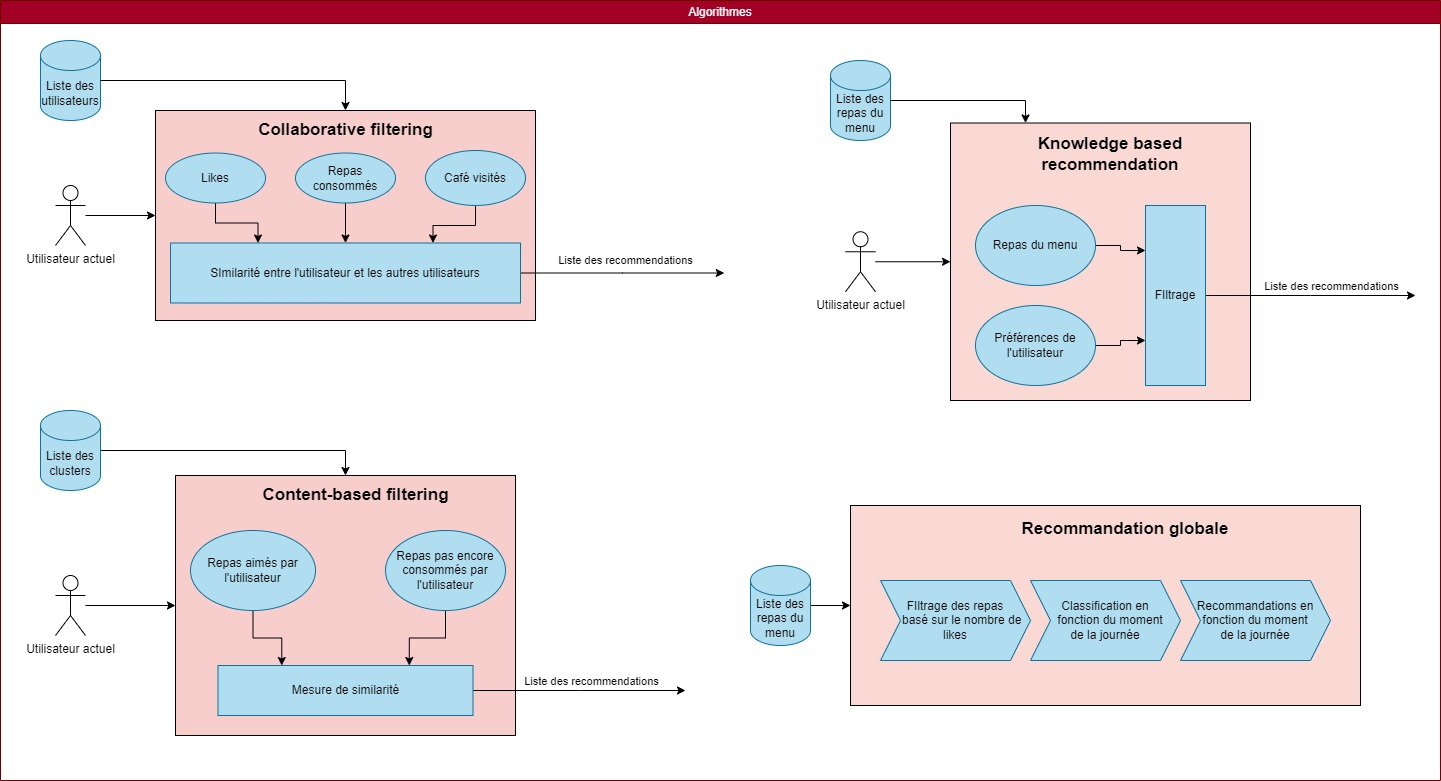
\includegraphics[scale=0.3]{Pipeline.jpg}
%\includesvg[scale=0.3]{Pipeline.drawio.svg}
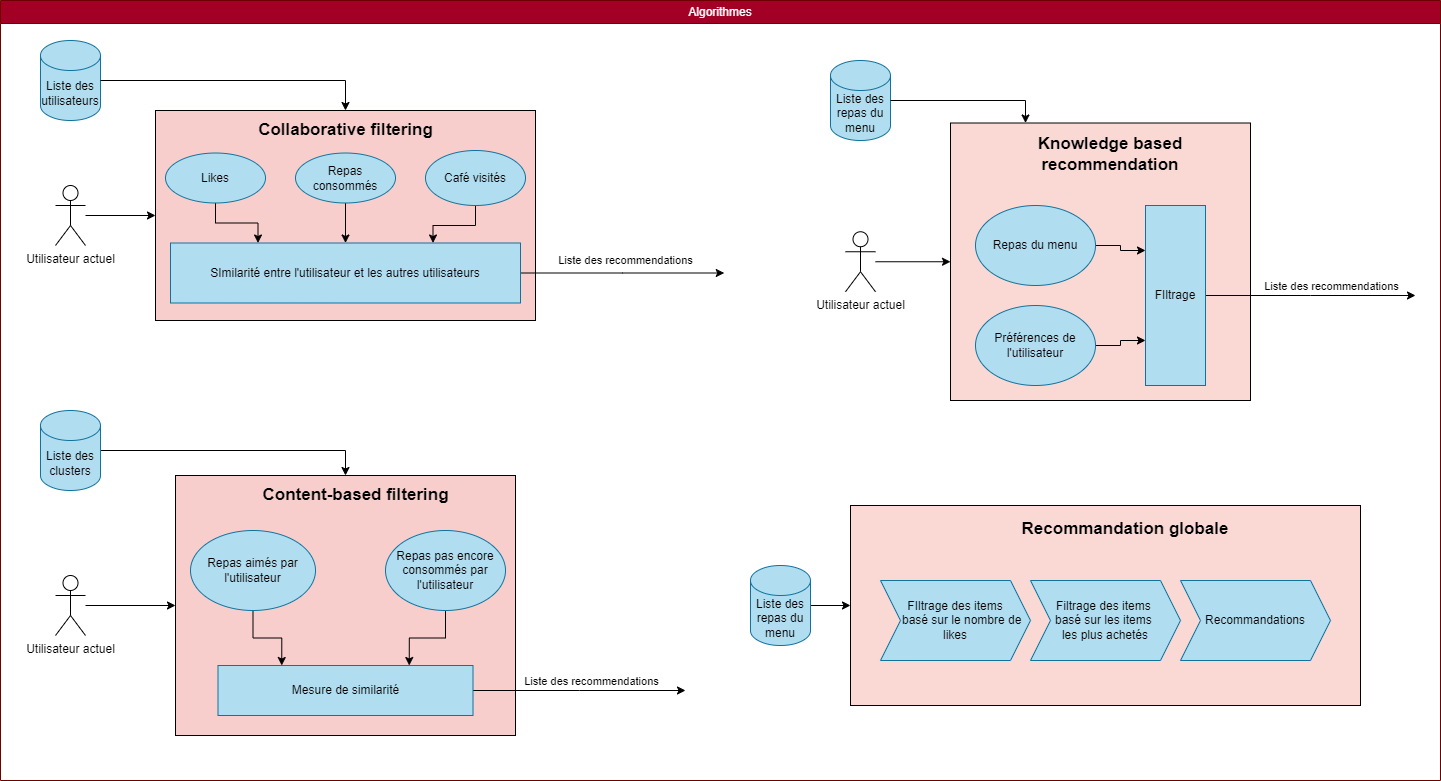
\includegraphics[scale=0.3]{images/Pipeline.drawio.png} 
\caption{Architecture des algorithmes}
\end{figure}

\subsection{Recommendation public (globales) d'items}
Les recommandations publiques s'adressent à toute la communauté étudiante ainsi que les professeurs. Elles se basent sur les items les plus aimés (likes) et les items les plus achetés par l'ensemble des utilisateurs. Ces recommandations sont affichées à titre indicatif pour l'utilisateur dans le sens où il pourra savoir, de façon global, qu'est-ce que les autres utilisateurs apprécient.\\

Cet algorithme fonctionne principalement par filtrage. En effet, pour un menu donné (un ensemble d'items), un premier filtrage est effectué en conservant uniquement les items possède le plus grand nombre de likes. Ensuite, parmi les items les plus aimés, un second filtrage est effectué pour conserver les items les plus achetés. Le nombre d'items conservé est limité à 10 pour ne pas surcharger l'interface au niveau du front-end. Voici un pseudo-code présentant le fonctionnement de l'algorithme:

\begin{algorithm}
    \caption{Recommandation globale}
    \begin{algorithmic}[1]
        \Statex \textbf{Description:} Recommandations à tout les utilisateurs.
        \Statex \textbf{Entrée:} Liste des repas du menu ($M$)
        \Statex \textbf{Sortie:} Liste des recommandations
        \State \textbf{\textit{Algorithme(M[1...n]):}}
        \State \hspace{0.5cm} $k \leftarrow$ nombre de repas à recommander
        \State \hspace{0.5cm} $I \leftarrow$ items les plus achetés
        \State \hspace{0.5cm} \textbf{retourner} $items\_plus\_aimes(I,k)$
        \\
--------------------------------------------------------------------------------------------------------------------
	\State \textbf{\textit{items\_plus\_aimes(I[1...n],k))}}:
	\State \hspace{0.5cm} $likes \leftarrow [vide]$
	\State \hspace{0.5cm} $res \leftarrow [vide]$
	\State \hspace{0.5cm} \textbf{Pour chaque} $item \in I$:
	\State \hspace{1cm} likes.insérer(item.likes.length)
	\State \hspace{0.5cm} \textbf{Pour} $i \leftarrow 0$ à $k$
	\State \hspace{1cm} $max\_like \leftarrow max(likes)$
	\State \hspace{1cm} $index \leftarrow likes.index(max\_likes)$ 
	\State \hspace{1cm} $res.inserer(I[index])$
	\State \hspace{1cm} $likes[index] \leftarrow -1$
	\State \hspace{0.5cm} \textbf{retourner} $res$
    \end{algorithmic}
\end{algorithm}

\newpage
\subsection{Recommandations personnalisées}
Contrairement aux recommandations publiques, les recommandations personnalisées sont spécifiquement adaptées à chaque utilisateur. Elles s’appuient sur les trois algorithmes présentés précédemment dans la \hyperref[2.2]{\textit{section 2.2}}. Les recommandations personnalisées se déclinent en deux catégories : les recommandations d'items et les recommandations de cafés. Le système de recommandations d'items suggère des articles aux utilisateurs en utilisant les trois algorithmes mentionnés. Pour les recommandations de cafés, le filtrage collaboratif est utilisé de manière similaire, à la différence que les \textit{outputs} des recommandations sont des cafés. Cependant, le filtrage basé sur le contenu est partiellement appliqué aux café alors que les recommandations basées sur les connaissances ne sont pas appliquées aux cafés.

\subsubsection{Filtrage Collaboratif}
Dans le cadre de \textit{Café sans-fil}, l'algorithme de filtrage collaboratif repose sur la similarité entre un utilisateur et les autres. La similarité entre deux utilisateurs est calculée en utilisant la \hyperref[jaccard]{\textit{similarité Jaccard}}. Les caractéristiques utilisées pour évaluer cette similarité incluent : les items aimés par l'utilisateur, les items achetés, et les cafés visités. Ces caractéristiques ont été sélectionnées, car elles reflètent fidèlement les habitudes de consommation propres à chaque utilisateur. Une fois la similarité calculée sur la base de ce vecteur d'attributs, seuls les utilisateurs présentant une similarité supérieure à un certain seuil sont retenus. Ce seuil est fixé à 60\% pour les données de test, mais il sera ajusté lors du déploiement sur des données réelles.\

Si un item acheté par un utilisateur sélectionné n'a pas encore été acheté par l'utilisateur cible, un score (correspondant à la similarité entre les deux utilisateurs) est attribué à cet item. Pour les recommandations de cafés, ce score est attribué au café. Voici un pseudo-code présentant le fonctionnement de l'algorithme:

\begin{algorithm}
    \caption{Collaborative filtering}
    \begin{algorithmic}[1]
        \Statex \textbf{Description:} Recommandations basées sur les similarités entre utilisateurs.
        \Statex \textbf{Entrée:} Liste des utilisateurs de l'application ($U$), utilisateur ($u$)
        \Statex \textbf{Sortie:} Liste $L$ des recommandations
        \State \textbf{\textit{Algorithme(U[1...n], u):}}
        \State \hspace{0.5cm} $L \leftarrow [vide]$
        \State \hspace{0.5cm} $\tau \leftarrow$ seuil de similarité 
        \State \hspace{0.5cm} $S \leftarrow U.retirer(u)$
        \State \hspace{0.5cm} $L_u \leftarrow$ [[u.likes], [u.repas\_consommés], [u.cafés\_visités]]
        \State \hspace{0.5cm} \textbf{Pour chaque} utilisateur $x\in S_{n\times 1}$
        \State \hspace{1cm} $L_x \leftarrow$ [[x.likes], [x.repas\_consommés], [x.cafés\_visités]]
        \State \hspace{1cm} $J \leftarrow [vide]$
        \State \hspace{1cm} \textbf{Pour} $i \leftarrow 0$ à $L_x.length$
        \State \hspace{1.5cm} $j \leftarrow Jaccard(L_u[i], L_x[i])$
        \State \hspace{1.5cm} $J.ajouter(j)$
        \State \hspace{1cm} $score \leftarrow sum(J)$
        \State \hspace{1cm} \textbf{Si} $score \geq \tau$:
        \State \hspace{1.5cm} $L \leftarrow (L_x[0] \cup L_x[1]) \backslash (L_u[0] \cup L_u[1])$
        \State \hspace{1cm} $S.retirer(x)$
        \State \hspace{0.5cm} \textbf{retourner} $L$
    \end{algorithmic}
\end{algorithm}

\subsubsection{Filtrage Basé sur le Contenu}
Dans le contexte de \textit{Café sans-fil}, les recommandations basées sur le contenu, en ce qui concerne les items, se fondent sur les groupes d'items les plus appréciés ainsi que sur la similarité entre ces items. Lors du prétraitement des données, les items sont regroupés en fonction de leur similarité à l'aide de l'algorithme de clustering \textit{KMeans}. Chaque cluster reçoit un score représentant le nombre d'items aimés par l'utilisateur dans ce cluster. Les clusters ayant le plus grand nombre de likes correspondent donc aux préférences de l'utilisateur. Ensuite, pour chaque cluster préféré, un score est attribué aux items de ce cluster que l'utilisateur n'a pas encore achetés, correspondant au score du cluster.\

En ce qui concerne les cafés, aucun clustering n'est effectué. Seuls les cafés offrant le plus d'items appréciés par l'utilisateur sont proposés. Dans ce cas, le score représente le nombre d'items aimés par l'utilisateur dans un café. Le pseudo-code de cet algorithme peut être retrouvé plus bas.

\begin{algorithm}
    \caption{Content based filtering}
    \begin{algorithmic}[1]
        \Statex \textbf{Description:} Recommandations basé sur les habitudes de consommation de l'utilisateur.
        \Statex \textbf{Entrée:} Menu du cafe ($M$), utilisateur ($u$)
        \Statex \textbf{Sortie:} Liste $L$ des recommandations
        \State \textbf{\textit{Algorithme(M[1...n], u):}}
        \State \hspace{0.5cm} $L \leftarrow [vide]$
        \State \hspace{0.5cm} $P \leftarrow$ Items pas encore achetés (\textbf{\textit{Algorithme 1}})
        \State \hspace{0.5cm} $clusters \leftarrow regrouper\_par\_cluster(M)$
        \State \hspace{0.5cm} $cf \leftarrow [vide]$
        \State \hspace{0.5cm} \textbf{Tant que} cf.length $<$ clusters.length:
        \State \hspace{1cm} $c \leftarrow cluster\_favoris(C, u)$
        \State \hspace{1cm} $cf.inserer(c)$
        \State \hspace{1cm} $C \leftarrow C.retirer(c)$
        \State \hspace{0.5cm} \textbf{Pour chaque} cluster $c$ $\in cf$:
        \State \hspace{1cm} $L.ajouter(P \cap c)$
        \State \hspace{0.5cm} \textbf{retourner} L
        \\
--------------------------------------------------------------------------------------------------------------------
        \State \textbf{\textit{cluster\_favoris(C[[1...n],[1...m],...k], u)}:}
        \State \hspace{0.5cm} $L \leftarrow [empty]$
        \State \hspace{0.5cm} \textbf{Pour chaque} cluster $c[1...n] \in C$:
        \State \hspace{1cm} $tmp \leftarrow [empty]$
        \State \hspace{1cm} \textbf{Pour chaque} repas $r \in c[1...n]$: 
        \State \hspace{2cm} \textbf{SI} $u \in r.likes$:
        \State \hspace{2.5cm} $tmp.ajouter(r)$
        \State \hspace{1cm} $L.ajouter(tmp.length)$
        \State \hspace{0.5cm} $i \leftarrow L.index\_du\_max$
        \State \hspace{0.5cm} \textbf{retourner} $C[i]$
        \\
--------------------------------------------------------------------------------------------------------------------
		\State \textbf{\textit{regrouper\_par\_cluster(M)}}:
		\State \hspace{0.5cm} $groupes \leftarrow \{vide\}$
		\State \hspace{0.5cm} \textbf{Pour chaque} item $\in M$:
		\State \hspace{1cm} \textbf{Si} $item.cluster \notin groupes$:
		\State \hspace{1.5cm} $groupes[item.cluster] = [vide]$
		\State \hspace{1cm} $groupes[item.cluster].inserer(item)$
		\State \hspace{0.5cm} \textbf{retourner} groupes 
		
    \end{algorithmic}
\end{algorithm}

\subsubsection{Recommandations Basées sur les Connaissances}
Tout comme les recommandations globales, les recommandations basées sur les connaissances fonctionnent par filtrage. Une interface utilisateur (profil nutritionnel) a été ajoutée pour collecter les préférences nutritionnelles des utilisateurs. Cette interface est présentée plus en détail dans la \hyperref[implementation]{\textit{section 4}}. À travers cette interface, il est possible de récupérer diverses préférences utilisateur telles que les régimes alimentaires suivis, les préférences nutritionnelles, et les allergies. Ensuite, les items du menu sont filtrés pour ne conserver que ceux compatibles avec le régime alimentaire choisi par l'utilisateur. Un second filtrage est appliqué pour respecter les autres préférences de l'utilisateur. Enfin, si certains items contiennent des allergènes de niveau 2 ou 3, ils sont retirés de la liste. Le pseudo-code de cet algorithme peut être retrouvé plus bas.

\begin{algorithm}
    \caption{Knowledge based filtering}
    \begin{algorithmic}[1]
        \Statex \textbf{Description:} Recommandations basé sur les spécifications de l'utilisateur.
        \Statex \textbf{Entrée:} Utilisateur actuel ($u$), Liste des repas du menu ($M$)
        \Statex \textbf{Sortie:} Liste des recommandations.
        \State \textbf{\textit{Algorithme(M[1...n], u):}}
        \State \hspace{0.5cm} $A \leftarrow u.liste\_allergens$
        \State \hspace{0.5cm} $allergenes \leftarrow repas\_allergens(A)$
        \State \hspace{0.5cm} $P \leftarrow u.preferences$
        \State \hspace{0.5cm} $R \leftarrow clusters(M)$ // \textbf{\textit{Algorithme 3}}
        \State \hspace{0.5cm} $E[0...n] \leftarrow$ récupérer les bons repas en fonction du régime (P[0]) et des
        \State \hspace{0.5cm} catégories (P[1]) spécifiées par l'utilisateur
        \State \hspace{0.5cm} \textbf{retourner} E
        \\
--------------------------------------------------------------------------------------------------------------------
        \State \textbf{\textit{repas\_allergenes(A[1...n], M[1...m]):}}
        \State \hspace{0.5cm} $L \leftarrow [vide]$
        \State \hspace{0.5cm} \textbf{Pour chaque} repas $r\in M$:
        \State \hspace{1cm} \textbf{Si} $r.allergens \cap A \neq \emptyset$:
        \State \hspace{1.5cm} $L$.inserer(r)
        %\State \hspace{0.5cm} Trier les repas de $L$ en fonction du niveau de gravité
        \State \hspace{0.5cm} \textbf{retourner} $L$
    \end{algorithmic}
\end{algorithm}

\subsubsection{Robot de Recommandation Santé}
Le robot de recommandation santé est conçu pour intégrer des items sains dans les recommandations personnalisées et publiques. Les items sont triés par ordre croissant de leur score santé (plus le score est bas, plus l'item est sain) et les items les plus sains sont ensuite intégrés aux recommandations. Cela vise à encourager la communauté étudiante à consommer davantage de produits sains.

\subsection{Score santé}
Les recommandations ne sont pas uniquement faites aux utilisateurs en se basant sur leur préférence et habitude de consommation. En effet, chaque item possède un score santé représentant à quel point cet item est bon pour la santé des utilisateurs. Ensuite, en prenant la moyenne arithmétique du score des items d'un café, on attribue un score café aux cafés. Le score utilisé pour les items est le \textit{Nutri-score} \cite{hercberg2021nutri}. Le pseudo-code peut être retrouvé plus bas.\\

\textbf{Nutri-score}\\

Le Nutri-Score est un système d'étiquetage nutritionnel visant à fournir une évaluation globale de la qualité nutritionnelle des aliments et boissons.\\

Il est basé sur un algorithme qui calcule un score nutritionnel global pour chaque produit. Ce score est déterminé en prenant en compte plusieurs critères nutritionnels, tels que :\\

\begin{itemize}
    \item[$\circ$] Éléments favorables : Les nutriments et composés bénéfiques pour la santé, tels que les fibres, les protéines, et les fruits et légumes. Plus la présence de ces éléments est élevée, plus le score est favorable.\\
    
    \item[$\circ$] Éléments défavorables : Les nutriments et composés potentiellement nocifs, comme les acides gras saturés, les sucres ajoutés et le sel. Plus la présence de ces éléments est élevée, plus le score est défavorable.\\
\end{itemize}

Le score final est calculé en soustrayant le total des points obtenus pour les éléments défavorables du total des points obtenus pour les éléments favorables. Lorsque le score est affiché aux consommateurs, ce dernier est ensuite converti en une lettre allant de \textbf{A} (meilleure qualité nutritionnelle) à \textbf{E} (moins bonne qualité nutritionnelle). Cependant, dans le projet, puisque ce score n'est pas affiché au grand publique, il est conservé en valeur décimal dans le but de faciliter les calculs effectués plus tard.\\

\textbf{Pourquoi le Nutri-score ?}\\

Plusieurs raisons justifient le choix de ce score:\\

\begin{itemize}

    \item[$\circ$] Standardisation : Le Nutri-Score offre un standard uniforme pour l'évaluation nutritionnelle, ce qui permet une comparaison cohérente entre différents produits, indépendamment des variations dans les étiquetages ou les allégations marketing.\\

    \item[$\circ$] Support pour les politiques de santé publique : En fournissant une information nutritionnelle transparente et accessible, le Nutri-Score soutient les initiatives de santé publique visant à réduire les maladies liées à l'alimentation et à promouvoir une meilleure santé globale.\\
\end{itemize}


\begin{algorithm}
	\caption{Health score}
	\begin{algorithmic}[1]
		\Statex \textbf{Description:} Calcul du score santé
		\Statex \textbf{Entrée:} item
		\Statex \textbf{Sortie:} Score
		
        \State \textbf{\textit{Health\_score(item):}}

		\State \hspace{0.5cm} negative\_points\_max $\gets$ 10 
		\State \hspace{0.5cm} positive\_points\_max $\gets$ 5

		\State \hspace{0.5cm} energy\_points $\gets$ \texttt{min}(\texttt{max}(item.calories / 335), 0), negative\_points\_max)
		\State \hspace{0.5cm} sugar\_points $\gets$ \texttt{min}(\texttt{max}(item.sugar / 4.5), 0), negative\_points\_max)
		\State \hspace{0.5cm} saturated\_fat\_points $\gets$ \texttt{min}(\texttt{max}(item.saturated\_fat / 1), 0), negative\_points\_max) 
		\State \hspace{0.5cm} sodium\_points $\gets$ \texttt{min}(\texttt{max}(item.sodium / 90), 0), negative\_points\_max)
		\State \hspace{0.5cm} negative\_points $\gets$ energy\_points + sugar\_points + saturated\_fat\_points + sodium\_points

		\State \hspace{0.5cm} fiber\_points $\gets$ \texttt{min}(\texttt{max}(item.fiber / 0.9), 0), positive\_points\_max)
		\State \hspace{0.5cm} protein\_points $\gets$ \texttt{min}(\texttt{max}(item.proteins / 1.6), 0), positive\_points\_max)
		\State \hspace{0.5cm} positive\_points $\gets$ fiber\_points + protein\_points

		\State \hspace{0.5cm} score $\gets$ negative\_points - positive\_points

		\State \hspace{0.5cm} \Return{score}
	\end{algorithmic}
\end{algorithm}


\newpage
\section{Implémentation}
\label{implementation}
\subsection{Spécification}
Cette section présente principalement les détails techniques de l'implémentation (principalement backend) propre au projet.

\subsubsection{Technologies}
Les technologies employées restent inchangées par rapport à celles déjà intégrées dans l'application web:
\textbf{Python} est utilisé pour la programmation côté serveur, \textbf{MongoDB} sert de base de données, \textbf{FastAPI} 
est utilisé pour le développement de l'API, \textbf{ReactJS} pour le développement de l'application (frontend) et 
\textbf{TailwindCSS} pour le style de l'application.\\


Deux nouvelles librairies ont été rajoutées dans le projet à savoir \textit{numpy} et \textit{sklearn}. C'est les librairies sont utilisées pour effectuer le clustering des items. Nous avons choisie choisi la librairie \textit{sklearn} car elle est l'une des plus populaires pour effectuer du clustering. De plus, elle possède précisément les méthodes dont nous avons besoin. La plupart des méthodes de \textit{sklearn} qui sont utilisées retournent des listes de type \textit{np.array} (numpy array) donc, l'utilisation de la librairie \textit{numpy} est nécessaire pour pouvoir utiliser \textit{sklearn}.

\subsubsection{Exécution}
Dans un premier temps, il faudrait tout d'abord exécuter les routines pour regrouper les items (clustering des items), assigner un score santé à ces items et également assigner un score santé aux cafés. Cela est nécessaire, car les algorithmes ont besoin du cluster et des score santé pour fonctionner. Ensuite, il n'y a pas d'ordre spécifique pour exécuter les algorithmes.\\

En raison du temps d'exécution assez long (à cause du manque d'optimisation présenté dans la \hyperref[discussion]{\textit{section 5.2}}), nous avons pensé temporairement retirer un algorithme (filtrage collaboratif), car, ce dernier prend le plus temps pour s'exécuter. En effet, les algorithmes de filtrage collaboratifs, filtrage basé sur le contenu et filtrage basé sur les connaissances, exécutés tous ensemble, prennent approximativement 2h30 pour produire des recommandations. L'algorithme de filtrage collaboratif contribue en grande à ce temps d'exécution. Ainsi, l'algorithme sera rajouté de nouveau après qu'il ait subi quelques modifications qui sont présentées dans la \hyperref[discussion]{\textit{section 5.2}}. En appliquant cette modification, les algorithmes sont planifiés être exécutés toutes les 2h environ.

\subsubsection{Base de données}
Une nouvelle base de données pour les recommandations a été créée. Elle contient essentiellement de nouveaux attributs propres aux recommandations:\\

\begin{itemize}
	\item[$\bullet$] \textbf{User recommendation}: Cette collection contient les recommandations personnalisées pour chaque utilisateur (recommandations d'items et de cafés) ainsi que les informations uniques à chaque utilisateur (nom d'utilisateur et identifiant).\\
	
	\item[$\bullet$] \textbf{Cafe for recommendation}: Cette collection contient la liste des recommandations publiques, le slug et le score santé de chaque café.\\
	
	\item[$\bullet$] \textbf{Items}: Cette collection contient l'identifiant, le slug, le score santé et le cluster de chaque item.\\
\end{itemize}

\subsubsection{API}
Au niveau de l'API, 13 endpoints ont été rajoutés pour gérer les recommandations.\\

\begin{itemize}
	\item[$\bullet$] \textbf{Cafe et Items}: Quatre endpoints ont été rajoutés pour pouvoir récupérer et modifier les informations (score santé, recommandations publiques) des cafés et des items.\\
	
	\item[$\bullet$] \textbf{Users}: Cinq endpoints ont été rajoutés pour récupérer un utilisateur, ses recommandations (recommandation de cafés et d'items) et modifier les recommandations.\\
	
	\item[$\bullet$] \textbf{Public}: Deux endpoints pour récupérer et modifier les recommandations publiques.\\
	
	\item[$\bullet$] \textbf{Bot}: Un endpoint a été rajouté pour récupérer les recommandations du robot de recommandations. Les recommandations sont calculées lors de l'appel de l'API donc, ces dernières ne sont pas stockées dans la base de données, ce qui justifie l'absence d'endpoints pour modifier les recommandations.\\
	
	\item[$\bullet$] \textbf{Gérant}: Un endpoint a été rajouté pour récupérer les items désirés par les utilisateurs, mais absents des cafés. \\
	
\end{itemize}

\subsection{Illustration}
Les modifications apportées dans le front-end se présentent à trois niveaux: l'ajout du profil nutritionnel, l'ajout de sections pour les recommandations publiques et personnalisées et l'ajout d'une section pour les recommandations de cafés personnalisés. Toutes les interfaces présentées plus bas peuvent être vu en \hyperref[images]{\textit{annexe}}.\\

\textbf{A. Profil nutritionnel}\\
\label{profileNutritionnel}
Le profil nutritionnel a été rajouté dans le but de pouvoir récupérer toutes les informations nécessaires pour pouvoir faire les recommandations basés sur les connaissances. Le profil est séparé en trois sections, mais les préférences nutritionnelles et les allergies sont regroupées ensemble, car elles sont similaires. \\

\begin{enumerate}
	\item \textbf{Régimes alimentaires}: Cette section permet à l'utilisateur de sélectionner un ou plusieurs régimes alimentaires qu'il souhaite. Initialement, trois régimes sont présents: Cétogène, Méditéranéen et Végétarien. Chaque régime possède un nom, une description (facultative), une liste d'ingrédients/aliments qui ne doivent pas être consommés dans le régime et une liste des items que l'utilisateur voudrait avoir dans le régime. Une fonctionnalité qui n'a pas pu être rajoutée à temps est l'affichage du nombre de cafés dans lesquels il existe des items respectant les spécifications du régime alimentaire. L'utilisateur a l'option de rajouter un nouveau régime alimentaire s'il le souhaite. Cependant, seuls les régimes que ce dernier a rajoutés sont éditables et supprimables. Les trois régimes affichés initialement ne sont ni éditables ni supprimables par l'utilisateur.\\
	
	 \item \textbf{Préférences nutritionnelles et allergies}: La section pour les préférences nutritionnelles permet à l'utilisateur de sélectionner les nutriments qu'il souhaite retrouver dans les aliments qui lui sont recommandés et à quelle proportion ils devraient se retrouver dans l'item (faible, moyen ou élevé). La section des allergies permet à l'utilisateur de sélectionner les aliments auquel il est allergique (lait/lactose, arachide/noix) et à quel degré ce dernier est allergique à ces aliments (faible, moyen, élevé).\\
\end{enumerate}

\textbf{B. Recommendation publique et personnalisée}\\
Pour l'affichage des recommandations publiques et personnalisées d'items, deux nouvelles boites ont été rajoutées dans le menu des cafés. Une boite "\textit{Pour moi}" contenant les items recommandés à l'utilisateur et une autre boite "\textit{Produits recommandés}" contenant les items recommandés à toute la communauté étudiante. La boite de recommandation personnalisée n'est visible que pour les utilisateurs qui sont connectés à l'application web.\\

\textbf{C. Recommendation de cafés}\\
L'affichage des recommandations de cafés se fait sur la page d'acceuil. En effet, une nouvelle section nommée "\textit{Recommendation}" a été rajoutée dans sur la page d'acceuil. Cette section contient les cafés qui ont été recommandés. Elle section n'est visible que pour les utilisateurs qui sont connectés à l'application web. En dessous de cette section se trouve la section "\textit{Tous les cafés}" qui contient tous les cafés de l'UdeM. Les cafés de cette section sont triés en fonction de leurs score santé afin que les cafés vendant les items les plus sains soient affichés en premiers.\\

\newpage


\section{Évaluation}
Pour s'assurer du bon fonctionnement des algorithmes intégrés à l'application web, des tests ont été effectués tout au long du développement. Les tests encourus sont divisés en 2 catégories:\\

\begin{itemize}
	\item[$\bullet$] \textbf{Tests fonctionnels (à la boite noire)}: Ils vérifient la conformité du code aux exigences en évaluant si les sorties correspondent aux attentes pour des entrées données, sans se soucier des détails internes du programme.\\
	
	\item[$\bullet$] \textbf{Tests d'utilisabilité}: Ils permettent de déterminer dans quelle mesure un produit ou un service (généralement une interface utilisateur ou un site web) est facile à utiliser pour les utilisateurs réels. Ces tests sont conçus pour identifier les problèmes d'utilisabilité, recueillir des données qualitatives et quantitatives, et améliorer l'expérience utilisateur.\\
\end{itemize}

Pour vérifier et valider que l'ajout de nouveaux endpoints ne provoque pas de changements indésirables dans l'application, une série de tests unitaires et de tests d'intégration a été réalisée.

\subsection{Tests}
La librairie \textit{unittest} de Python a été choisie pour effectuer les tests unitaires en raison de sa simplicité d'utilisation et de mon expérience antérieure avec cet outil.

\subsubsection{Tests unitaires}
Un total de 74 tests unitaires ont été réalisés. Environ 63 tests ont été créés pour garantir le bon fonctionnement des algorithmes, et 10 autres pour vérifier le bon fonctionnement des nouveaux endpoints de l'API. Les tests API sont structurés de manière cohérente avec ceux déjà en place.\\

Les tests des algorithmes sont structurés comme suit :
\begin{enumerate}
	\item Chaque script contenant les tests d'un algorithme est subdivisé en \textit{class}. Chaque \textit{class} contient les différents tests correspondant à une méthode intermédiaire utilisée dans l'algorithme. Ainsi, chaque méthode dans la \textit{class} s'assure de tester d'une ou de plus manière la fonction à tester. L'algorithme possède aussi une \textit{class} contenant ses tests. Si des méthodes intermédiaires ne nécessitent qu'un seul cas de test, ces dernières sont incluses dans la même \textit{class} de test que l'algorithme principal.\\
	
	\item Dans le but de contrôler le mieux possible l'environnement de test, les mocks sont utilisées pour éviter de biaiser le fonctionnement des algorithmes. Ainsi, ces derniers sont utilisés uniquement sur les méthodes faisant appel à l'API. Cela permet de s'assurer que si un test échoue, l'erreur est uniquement liée à l'algorithme lui-même ou à son implémentation et non à un problème au niveau de l'API.\\
	
	\item Chaque \textit{class} de test contient, si nécessaire, une méthode \textit{setUp} qui permet d'initialiser les objets utilisés par plusieurs tests. Si un objet spécifique est requis pour faire un test et qu'il n'est requis que pour ce test, il est rajouté uniquement dans la méthode test.\\
	
	\item Les tests unitaires suivent le style \textbf{AAA}: \textbf{Arrange} (section du test initialisant les objets utilisés par la méthode à tester), \textbf{Act} (section où l’on invoque la méthode testée avec les paramètres créés précédemment) et \textbf{Assert} (section vérifiant que la méthode produit le comportement désiré).\\
\end{enumerate}

La figure ci-dessous est un test unitaire vérifiant que l'algorithme de filtrage basé sur le contenu retourne bien les items qu'il devrait retourner dans le cas où un utilisateur a déjà acheté tous les items d'un café.

\begin{lstlisting}[language=Python, caption=Test unitaire test\_main\_4 content based filtering]
class TestContentBasedFiltering(unittest.TestCase):
    def setUp(self):
        self.user1 = {'user_id': 'user1', 'username': 'username1'}
        self.cafes = [
            # Cafe1 doesn't contain user2
            {
                'slug': 'cafe1',
                'menu_items': [
                    {'slug': 'item1', 'likes': []}, 
                    {'slug': 'item2', 'likes': ['user1']},
                    ...
                ]
            }, 
			...
    # autres methodes de la classe
    @patch('recommender_systems.utils.api_calls.CafeApi.get_all_items')
    @patch('recommender_systems.utils.db_utils.get_user_likes_in_cafe')
    @patch('recommender_systems.utils.utilitaries.items_not_bought_in_cafe')
    def test_main_4(self, mock_items_not_bought_in_cafe, mock_get_user_likes, mock_api_get_all_items):
        # ARRANGE: Recuperation des objets de la methode setUP
        user = self.user1
        cafe = self.cafes[0]

        # Mock d'un appel de l'API
        mock_api_get_all_items.return_value = ([
            {'slug': 'item1', 'likes': []}, 
            {'slug': 'item2', 'likes': ['user1']},
            {'slug': 'item3', 'likes': ['user5', 'user3']},
            ...
        ], 200)

        # Mocking
        mock_items_not_bought_in_cafe.return_value = set()
        mock_get_user_likes.return_value = ['item2', 'item4']
        
        # ACT et ASSERT
        self.assertCountEqual(main(user, cafe), ['item2', 'item4'])

        # Mocking
        mock_get_user_likes.return_value = []
        mock_items_not_bought_in_cafe.return_value = set()

        # ACT et ASSERT
        self.assertCountEqual(main(user, cafe), ['item5', 'item4', 'item3', 'item2', 'item1'])
\end{lstlisting}

\subsubsection{Tests d'utilisabilité}
Une fois une première version de l'interface pour le profil nutritionnel complétée, des tests d'utilisabilité ont été réalisés. Lors d'une foire aux projets qui s'est tenue le jeudi 25 juillet, il a été possible de recueillir des retours de la part des autres étudiants, ce qui a permis d'améliorer la présentation de l'interface utilisateur ainsi que l'expérience utilisateur du profil.\

De plus, j'ai présenté l'application à certains membres de ma famille peu familiers avec les outils informatiques, dans le but d'obtenir des retours plus diversifiés. Ces commentaires ont été très pertinents pour améliorer l'expérience utilisateur de l'interface initiale.\

Un commentaire fréquemment revenu concernait le manque d'animations dans le profil, qui sera une piste d'amélioration pour l'avenir.

\subsection{Discussion}
\label{discussion}
Cette section est dédiée à effectuer des remarques et critiques sur les algorithmes. Les critiques seront effectuées par rapport à l'optimalité (complexité et Scalabilité) et la robustesse de l'algorithme. Puisque les algorithmes de recommandation des cafés sont très similaires aux algorithmes de recommandations personnelles, les critiques de ces dernières sont aussi valables pour les cafés.

\subsubsection{Filtrage collaboratif}
\begin{itemize}
	\item[$\bullet$] \textbf{Complexité temporelle:} Cet algorithme calcule la similarité entre l'utilisateur cible et tous les autres utilisateurs, ce qui peut entraîner une complexité de l'ordre de $O(n \times m)$, où $n$ est le nombre d'utilisateurs et $m$ est le nombre d'attributs comparés. Bien que cette approche soit fonctionnelle pour des jeux de données de taille modérée, elle devient peu optimale lorsque le nombre d'utilisateurs augmente significativement. Pour des systèmes à grande échelle comme l'\textit{UdeM} (l'université contient environ 67000 étudiants !), cela pourrait ralentir les performances, nécessitant potentiellement des techniques de réduction de la dimensionnalité comme les méthodes \textit{PCA} et \textit{MDS} pour réduire les nombres d'éléments à comparer lors du calcul de la similarité tout en conservant le plus d'information dans les données. En effet, l'utilisation de la similarité jaccard donne des résultats précis, mais cet algorithme devient moins efficace pour de larges données. L'utilisation des méthodes de clustering comme \textit{KMeans} pour regrouper les utilisateurs permettrait aussi d'améliorer significativement l'efficacité. \\
	
	\item[$\bullet$] \textbf{Scalabilité:} Comme mentionné précédemment, cet algorithme peut rencontrer des difficultés à s'adapter à un grand nombre d'utilisateurs ou de données en raison de la nécessité de calculer des similarités entre chaque paire d'utilisateurs. Dans les cas où le nombre d'utilisateurs est très élevé, des approches alternatives comme le filtrage collaboratif basé sur des modèles (qui se trouve dans la famille des recommandations basée sur les models) seraient plus efficaces.\\
	
	\item[$\bullet$] \textbf{Robustesse:} Les différents scénarios possibles sont pris en compte par l'algorithme, mais une meilleure gestion des erreurs et des exceptions, notamment en ajoutant des logs plus détaillés, améliorerait sa robustesse et faciliterait le débogage.\\
	
	\item[$\bullet$] \textbf{Réutilisabilité:} L'algorithme est étroitement couplé avec des appels à des utilitaires spécifiques, ce qui pourrait limiter sa réutilisabilité dans d'autres contextes ou projets. Une approche consistant à abstraire ces dépendances rendrait l'algorithme plus modulaire et adaptable à différents environnements ou bases de données.\\
	
	\item[$\bullet$] \textbf{Extensibilité:} L'algorithme pourrait être plus flexible en permettant l'utilisation de différentes métriques de similarité ou en adaptant dynamiquement le seuil de similarité en fonction des besoins spécifiques de l'utilisateur ou du contexte.\\
	
\end{itemize}

En somme, pour une potentielle amélioration de l'algorithme, il faudrait donc diminuer la dépendance de l'algorithme à d'autres modules de l'application, utiliser des méthodes de clustering ou de réduction de dimensionnalité pour augmenter son efficacité et afficher des logs plus détaillés pour faciliter la maintenance des algorithmes.

\subsubsection{Filtrage basé sur le contenu}

\begin{itemize}
	\item[$\bullet$] \textbf{Complexité temporelle:} L'algorithme regroupe les items en clusters et itère sur ces derniers pour trouver ceux que l'utilisateur a le plus appréciés. La complexité de cette opération dépend du nombre de clusters et d'items par cluster. Similairement à l'algorithme de filtrage collaboratif, cette méthode pourrait rencontrer des problèmes de performance lorsque le nombre de clusters ou d'items est très élevé. L'utilisation d'une approche de prétraitement, comme l'indexation inversée, pourrait potentiellement réduire les coûts de recherche.\\
	
	\item[$\bullet$] \textbf{Scalabilité:} Le processus de sélection des clusters les plus appréciés pourrait être optimisé en précalculant et en stockant les résultats des préférences de l'utilisateur, plutôt que de les recalculer à chaque exécution de l'algorithme. Donc, il serait plus efficace de créer une routine qui calculerait les clusters favoris de l'utilisateur et qui les mettrait à jour dans la base de données.\\
	
	\item[$\bullet$] \textbf{Robustesse:} Comme pour le filtrage collaboratif, l'ajout de logs plus détaillés permettront faciliteront le débogage et augmenteront la robustesse de l'algorithme.\\

	\item[$\bullet$] \textbf{Réutilisabilité:} L'algorithme est assez spécifique dans l'ensemble même si certaines composantes (script pour trouver les clusters favoris par exemple) peuvent être réutilisées dans d'autres contextes.\\
		
\end{itemize}

En somme, l'utilisation d'indexage inversé, la réduction de la dépendance de l'algorithme avec d'autres modules de l'application ainsi l'ajout de meilleurs logs pour le débogage serait des modifications qui améliorerait l'algorithme dans son ensemble.

\subsubsection{Filtrage basé sur les connaissances}

\begin{itemize}
	\item[$\bullet$] \textbf{Complexité temporelle et scalabilitée:} La complexité temporelle est de l'ordre de $O(n \times m \times k)$ dans le pire cas (l'utilisateur spécifie des préférences nutritives et des régimes alimentaires) où $n$ est le nombre d'items, $m$, le nombre de régimes alimentaires et $k$, le nombre de filtrages appliqués. Cet algorithme est acceptable avec une quantité faible ou moyenne de données, mais, lorsque le nombre de données est élevé, la performance de l'algorithme pourrait significativement diminuer en raison des multiples filtrages qui sont appliqués. L'algorithme pourrait être amélioré en utilisant davantage des structures de données appropriées (les ensembles et dictionnaires), en évitant les calculs répétitifs (comme les comparaisons redondantes) et en réduisant le nombre d'opérations coûteuses.\\
		
	\item[$\bullet$] \textbf{Robustesse et réutilisabilité :} Les commentaires faits aux algorithmes précédents s'appliquent aussi à cet algorithme.\\
	
	\item[$\bullet$] \textbf{Extensibilité:} Le point fort de cet algorithme serait son extensibilité en ce sens qu'il est très facile de rajouter de nouveaux filtres. Cependant, il serait quand même plus intéressant pour faciliter l'ajout de nouveaux filtres, de regrouper les différents filtres dans un script différent de celui de l'algorithme.\\
	
\end{itemize}

En résumé, cet algorithme souffre des mêmes problèmes de robustesse et de réutilisabilité que les autres algorithmes en ce sens qu'il dépend beaucoup trop des modules spécifiques à l'application web \textit{Café sans-fil}. L'algorithme serait donc plus optimal dans l'ensemble en réduisant la dépendance avec d'autres modules de l'application et en ajoutant de meilleurs logs pour le débogage.

\section{Conclusion}
Ce rapport a présenté une approche complète pour le développement d'un système de recommandation de repas personnalisé, en tenant compte des préférences nutritionnelles, des restrictions alimentaires, et des préférences de l'utilisateur. Les différentes sections ont mis en lumière l'importance de l'intégration de multiples algorithmes, chacun étant conçu pour optimiser un aspect spécifique du processus de recommandation. L'utilisation d'algorithmes de filtrage collaboratif, de filtrage basé sur le contenu, et de recommandations basées sur la connaissance a permis de créer un système robuste capable de s'adapter aux besoins variés des utilisateurs.\\

Les tests d'utilisabilité effectués ont permis d'affiner l'interface utilisateur, rendant le système plus intuitif et accessible. Les retours des utilisateurs ont été essentiels pour identifier des pistes d'amélioration, notamment l'intégration d'animations et d'améliorations visuelles pour enrichir l'expérience utilisateur.\\

Enfin, les critiques apportées aux algorithmes, en termes de complexité, scalabilité, et robustesse, ont permis de souligner les points forts et les défis à relever dans l'avenir. L'optimalité des algorithmes, bien que satisfaisante dans le cadre actuel, pourrait bénéficier de futures optimisations pour traiter des jeux de données plus vastes et diversifiés.\\

En conclusion, ce travail jette les bases d'une application de recommandation alimentaire personnalisée, avec un potentiel d'évolution et d'adaptation pour répondre aux nouvelles exigences des utilisateurs et du marché. Les prochaines étapes incluront l'amélioration continue des algorithmes et l'intégration de nouvelles fonctionnalités pour mieux servir les utilisateurs et enrichir leur expérience.

\section*{Remerciement}
Il est important de mentionner que ce projet n’aurait pas vu le jour sans le support de \textbf{l’Université de 
Montréal} et plus précisément, \textbf{Louis-Édouard LAFONTANT}, qui a supervisé et fourni une 
précieuse aide durant le développement et \textbf{Dr. Stefan Monnier}, PhD qui chapeaute ce cours et a accepté de me 
laisser poursuivre ce projet pendant la session.

\newpage
\bibliographystyle{ieeetr}
\bibliography{references}% common bib file

\section*{Annexe}

\subsection*{Images de l'implémentation du front}
\label{images}

\begin{figure}[H]
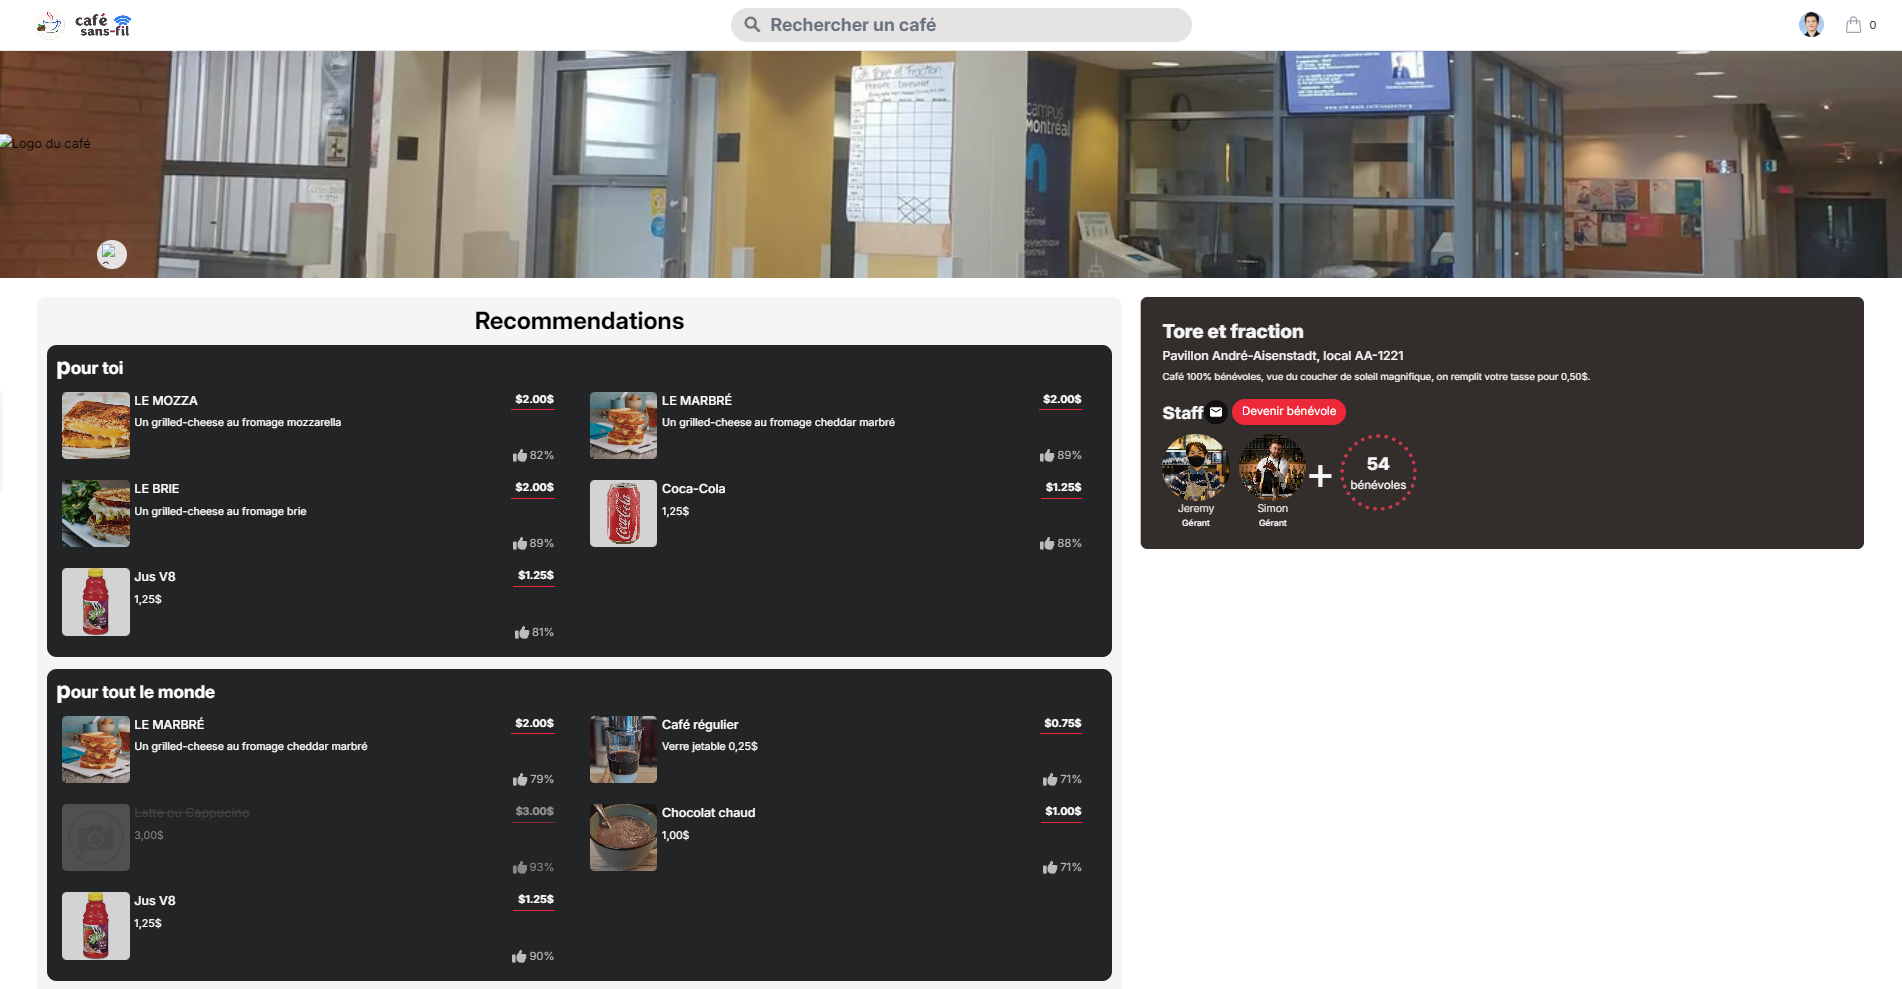
\includegraphics[scale=0.3]{images/recommendation_personnalises.png} \\
%\caption{Recommendation personnalisés et publiques}

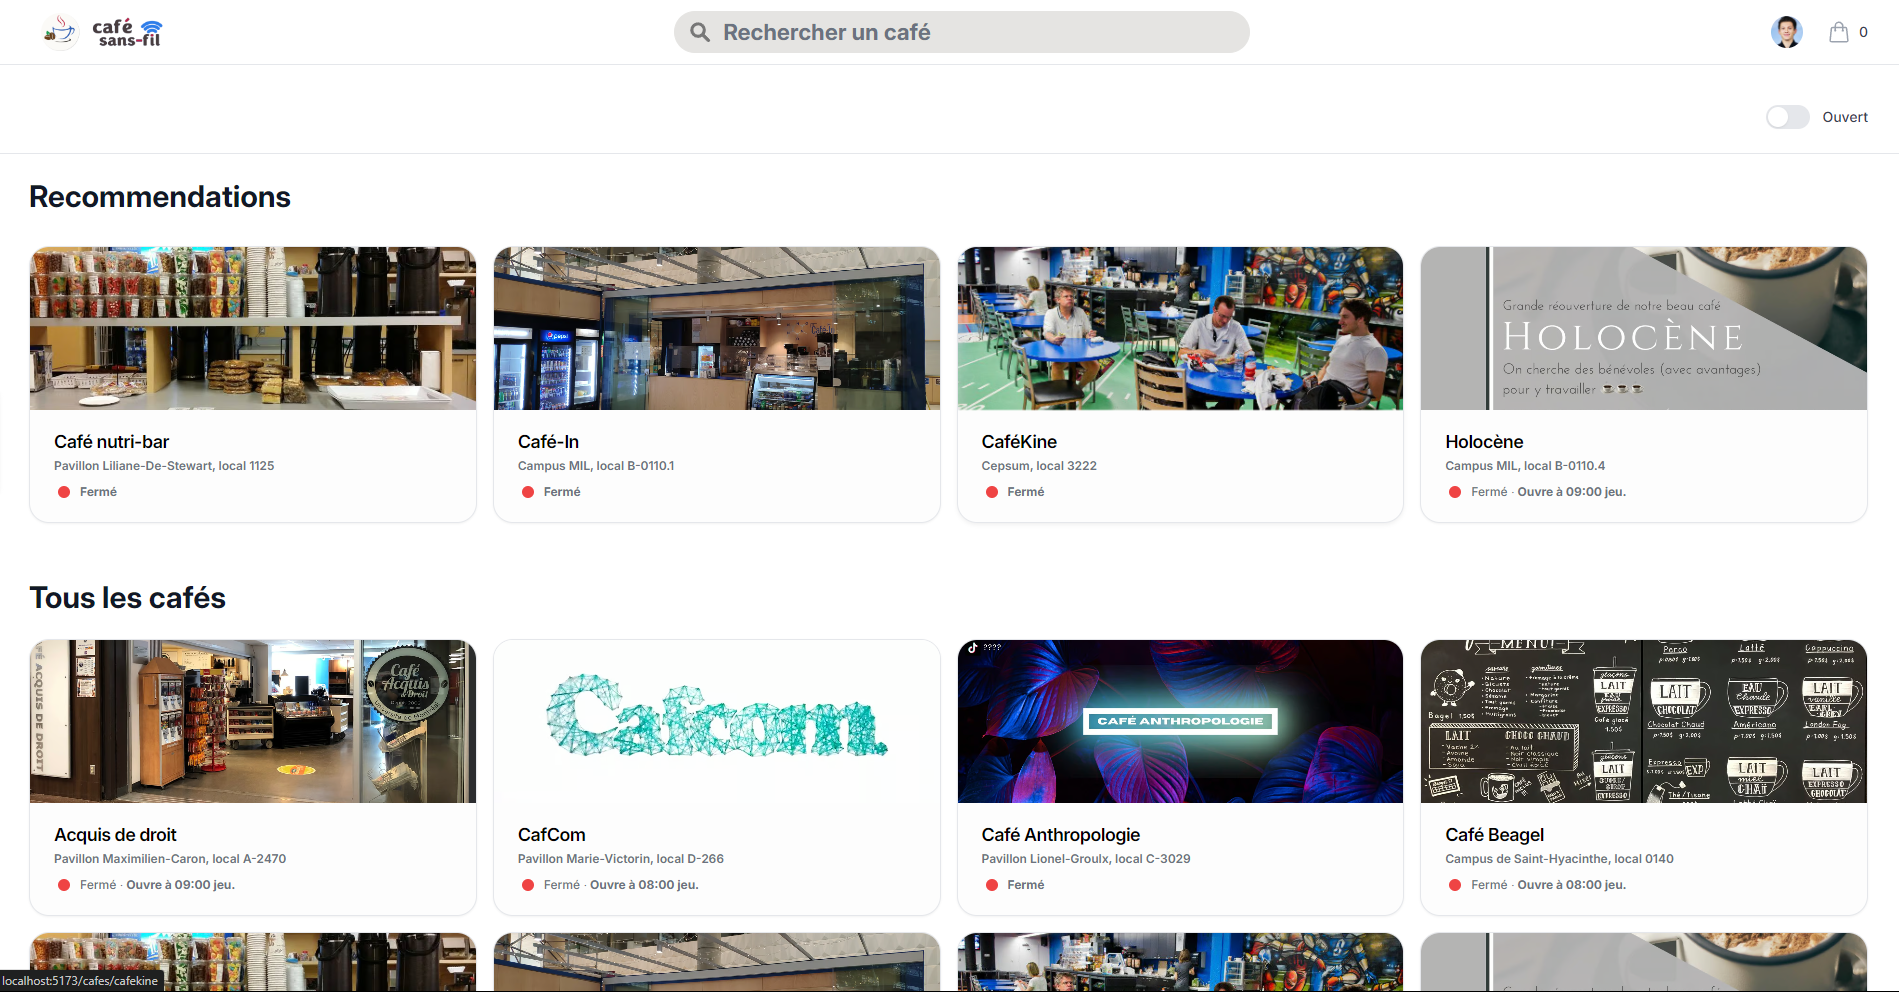
\includegraphics[scale=0.3]{images/recommendation_cafe.png} \\
%\caption{Recommendation des cafés}

\caption{Images des recommandations}
\end{figure}

\begin{figure}[H]
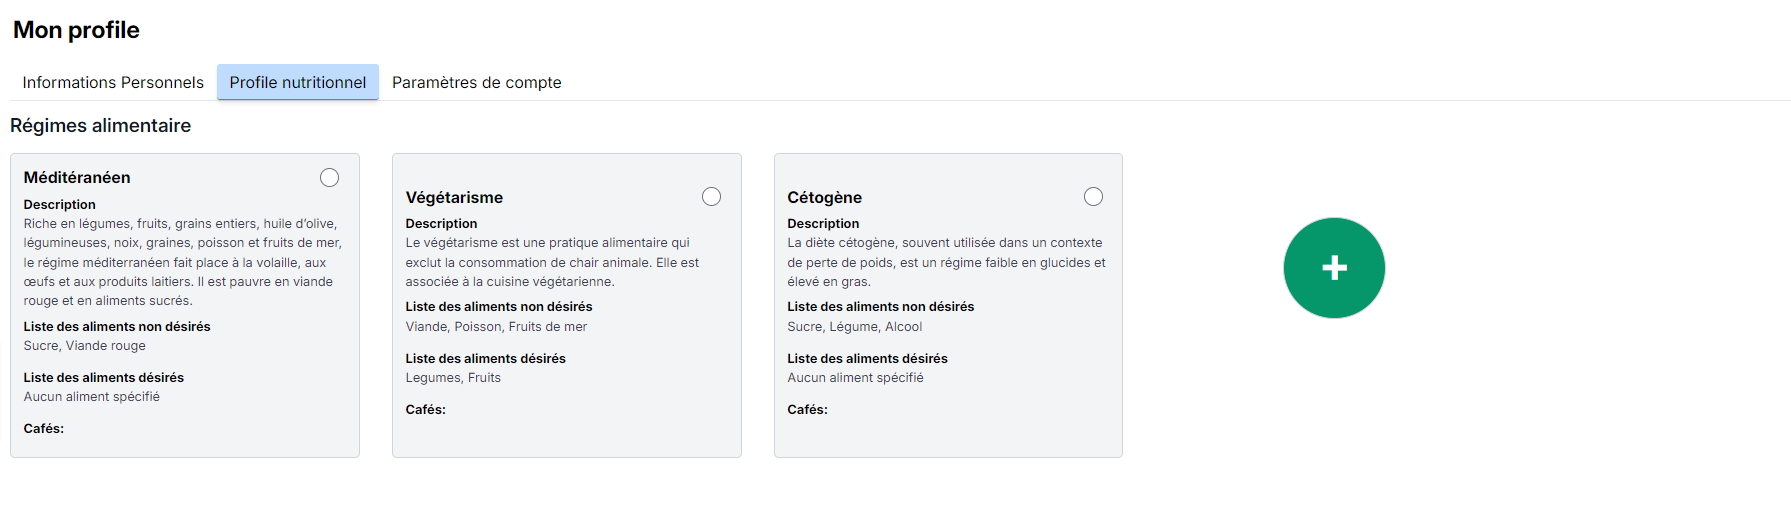
\includegraphics[scale=0.4]{images/diet_profile.png} \\
%\caption{Régime alimentaires}

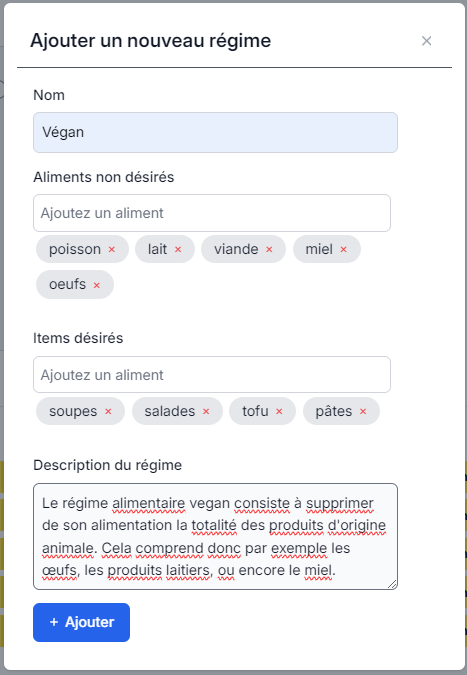
\includegraphics[scale=0.5]{images/add_new_diet.png} \\
%\caption{Ajout d'un nouveau régime}

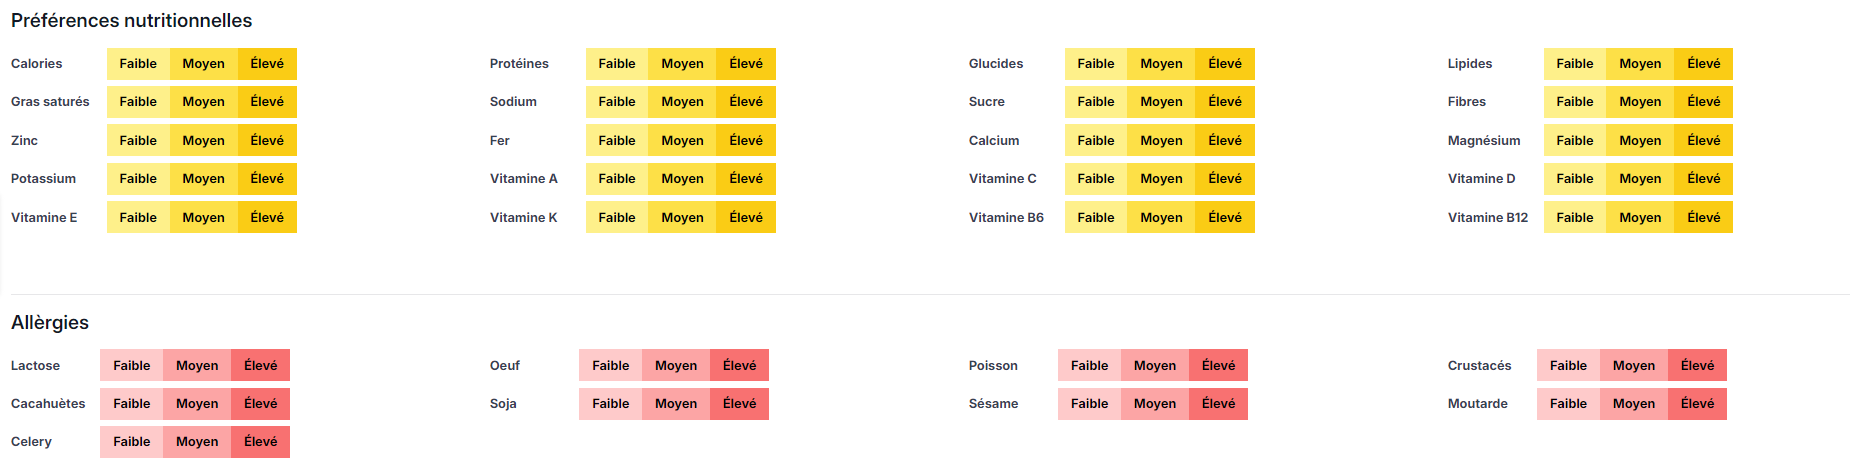
\includegraphics[scale=0.5]{images/preferences_allergenes.png} \\
%\caption{Préférences nutionnelles et allergènes}

\caption{Image du profil nutritionnel}
\end{figure}

\begin{figure}[H]
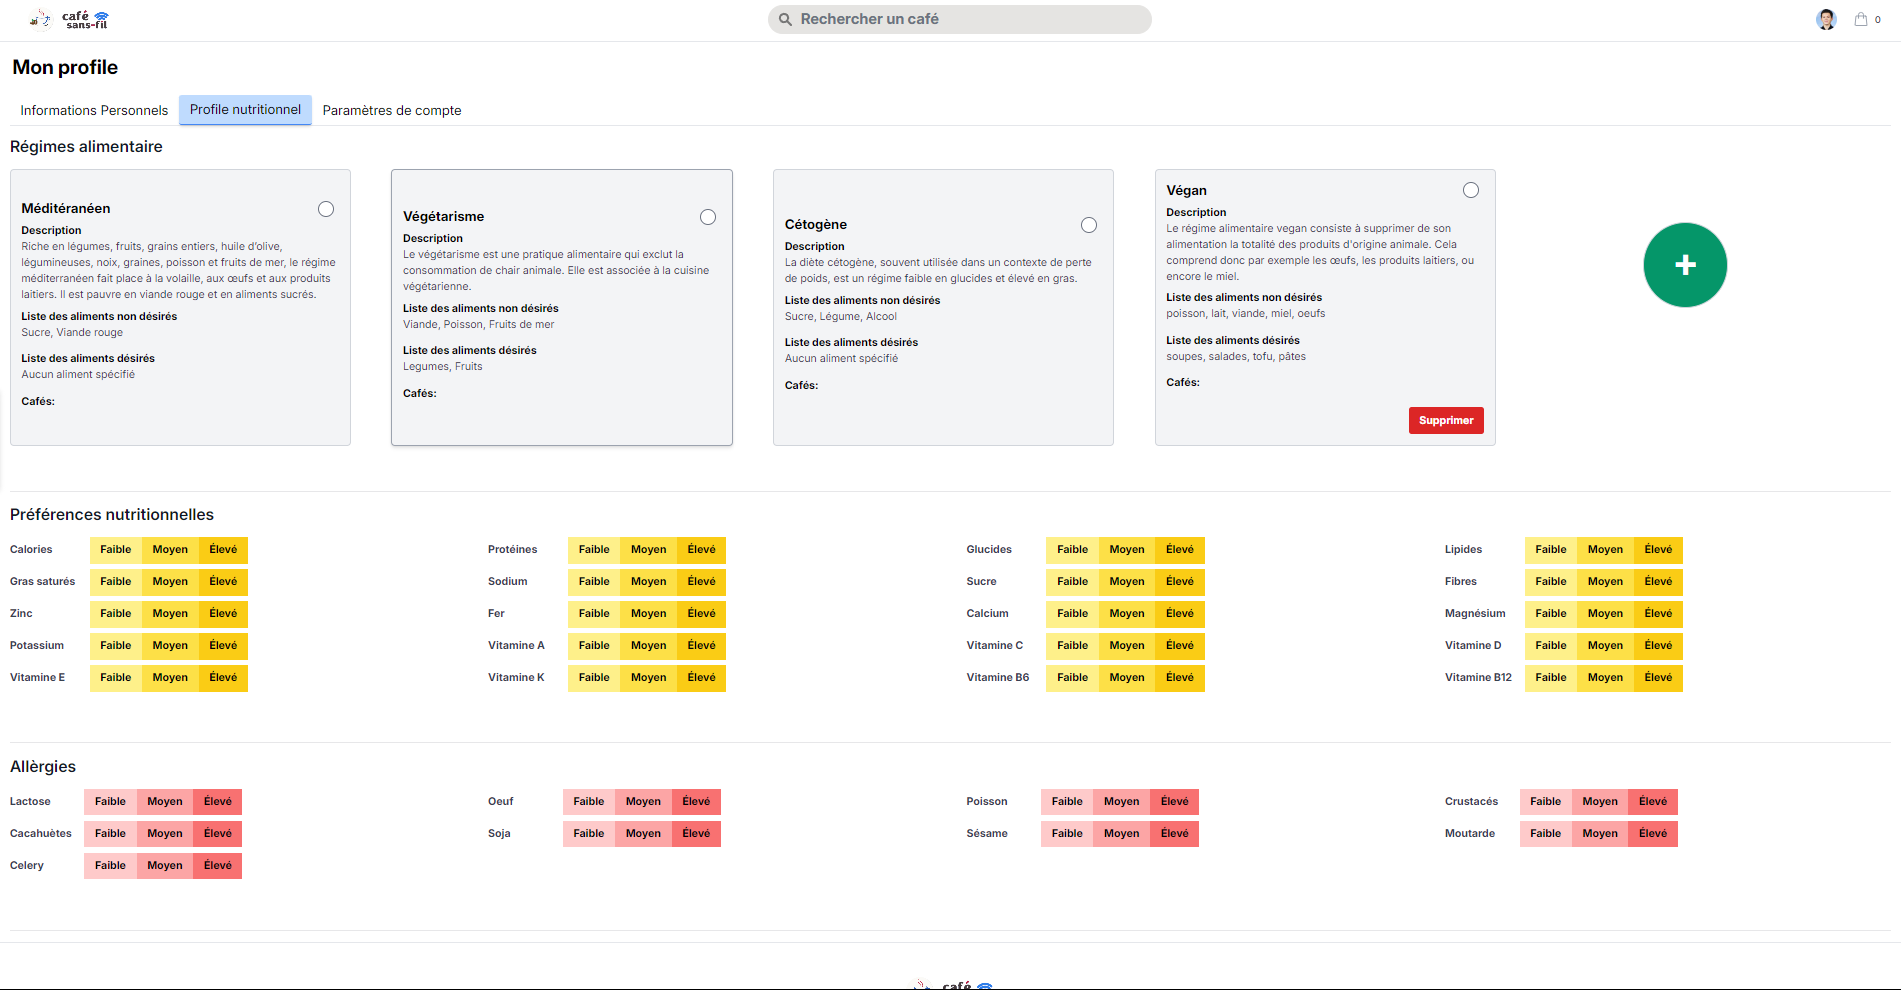
\includegraphics[scale=0.35]{images/full_profile.png}
\caption{Image complète du profil}
\end{figure}
 

\subsection*{Méthodes utilitaires}
\label{annexe}
\begin{algorithm}[H]
    \caption{Repas pas encore consommés}
    \begin{algorithmic}[1]
    \Statex \textbf{Entrée:} Menu du restaurant ($M$), utilisateur actuel ($u$)
    \Statex \textbf{Sortie:} Liste de repas
    \State \textbf{\textit{Algorithme(M[1...n], u)}}
    \State \hspace{0.5cm} $L \leftarrow u.historique\_achat$
    \State \hspace{0.5cm} \textbf{Pour chaque} repas $r \in L$
    \State \hspace{1cm} \textbf{Si} $r \in M$:
    \State \hspace{1.5cm} $M.retirer(r)$
    \State \hspace{0.5cm} \textbf{retourner} $M$
    \end{algorithmic}
\end{algorithm}

\begin{algorithm}[H]
    \caption{Mesure similarité: Jaccard}
    \begin{algorithmic}[1]
    \Statex \textbf{Entrée:} Deux listes ou ensembles ($L_1, L_2$)
    \Statex \textbf{Sortie:} Nombre décimal représentant la similarité
    \State \textbf{\textit{Jaccard($L_1[1...n]$,$L_2[1...m]$):}}
    \State \hspace{0.5cm} $union \leftarrow L_1 \cup L_2$
    \State \hspace{0.5cm} $inter \leftarrow L_1 \cap L_2$
    \State \hspace{0.5cm} \textbf{retourner} $inter.length/union.length$
    \end{algorithmic}
\end{algorithm}

\begin{algorithm}[H]
    \caption{Clusters en fonction des préférences de l'utilisateur}
    \begin{algorithmic}[1]
    \Statex \textbf{Entrée:} Menu du restaurant ($M$)
    \Statex \textbf{Sortie:} Liste des régimes contenant les catégories de repas
    \State \textbf{\textit{clusters(M[1...n])}}
    \State \hspace{0.5cm} // Nous avons k régimes différents et p catégories de repas
    \State \hspace{0.5cm} $R \leftarrow [[0...n]...k]$
    \State \hspace{0.5cm} \textbf{Pour chaque} repas $r \in M$:
    \State \hspace{1cm} mettre le repas dans un ensemble en fonction de son régime
    \State \hspace{1cm} rajouter les différents régimes de repas à $R$
    \State \hspace{0.5cm} \textbf{Pour chaque} régime $T[1...\ell] \in R$ 
    \State \hspace{1cm} mettre chaque repas du même régime dans une catégorie 
    \State \hspace{0.5cm} \textbf{retourner} $R[[[0...n]...p]...k]$
    \end{algorithmic}
\end{algorithm}

\end{document}
